% Options for packages loaded elsewhere
\PassOptionsToPackage{unicode}{hyperref}
\PassOptionsToPackage{hyphens}{url}
%
\documentclass[
]{article}
\usepackage{lmodern}
\usepackage{amssymb,amsmath}
\usepackage{ifxetex,ifluatex}
\ifnum 0\ifxetex 1\fi\ifluatex 1\fi=0 % if pdftex
  \usepackage[T1]{fontenc}
  \usepackage[utf8]{inputenc}
  \usepackage{textcomp} % provide euro and other symbols
\else % if luatex or xetex
  \usepackage{unicode-math}
  \defaultfontfeatures{Scale=MatchLowercase}
  \defaultfontfeatures[\rmfamily]{Ligatures=TeX,Scale=1}
\fi
% Use upquote if available, for straight quotes in verbatim environments
\IfFileExists{upquote.sty}{\usepackage{upquote}}{}
\IfFileExists{microtype.sty}{% use microtype if available
  \usepackage[]{microtype}
  \UseMicrotypeSet[protrusion]{basicmath} % disable protrusion for tt fonts
}{}
\makeatletter
\@ifundefined{KOMAClassName}{% if non-KOMA class
  \IfFileExists{parskip.sty}{%
    \usepackage{parskip}
  }{% else
    \setlength{\parindent}{0pt}
    \setlength{\parskip}{6pt plus 2pt minus 1pt}}
}{% if KOMA class
  \KOMAoptions{parskip=half}}
\makeatother
\usepackage{xcolor}
\IfFileExists{xurl.sty}{\usepackage{xurl}}{} % add URL line breaks if available
\IfFileExists{bookmark.sty}{\usepackage{bookmark}}{\usepackage{hyperref}}
\hypersetup{
  hidelinks,
  pdfcreator={LaTeX via pandoc}}
\urlstyle{same} % disable monospaced font for URLs
\usepackage[margin=1in]{geometry}
\usepackage{color}
\usepackage{fancyvrb}
\newcommand{\VerbBar}{|}
\newcommand{\VERB}{\Verb[commandchars=\\\{\}]}
\DefineVerbatimEnvironment{Highlighting}{Verbatim}{commandchars=\\\{\}}
% Add ',fontsize=\small' for more characters per line
\usepackage{framed}
\definecolor{shadecolor}{RGB}{248,248,248}
\newenvironment{Shaded}{\begin{snugshade}}{\end{snugshade}}
\newcommand{\AlertTok}[1]{\textcolor[rgb]{0.94,0.16,0.16}{#1}}
\newcommand{\AnnotationTok}[1]{\textcolor[rgb]{0.56,0.35,0.01}{\textbf{\textit{#1}}}}
\newcommand{\AttributeTok}[1]{\textcolor[rgb]{0.77,0.63,0.00}{#1}}
\newcommand{\BaseNTok}[1]{\textcolor[rgb]{0.00,0.00,0.81}{#1}}
\newcommand{\BuiltInTok}[1]{#1}
\newcommand{\CharTok}[1]{\textcolor[rgb]{0.31,0.60,0.02}{#1}}
\newcommand{\CommentTok}[1]{\textcolor[rgb]{0.56,0.35,0.01}{\textit{#1}}}
\newcommand{\CommentVarTok}[1]{\textcolor[rgb]{0.56,0.35,0.01}{\textbf{\textit{#1}}}}
\newcommand{\ConstantTok}[1]{\textcolor[rgb]{0.00,0.00,0.00}{#1}}
\newcommand{\ControlFlowTok}[1]{\textcolor[rgb]{0.13,0.29,0.53}{\textbf{#1}}}
\newcommand{\DataTypeTok}[1]{\textcolor[rgb]{0.13,0.29,0.53}{#1}}
\newcommand{\DecValTok}[1]{\textcolor[rgb]{0.00,0.00,0.81}{#1}}
\newcommand{\DocumentationTok}[1]{\textcolor[rgb]{0.56,0.35,0.01}{\textbf{\textit{#1}}}}
\newcommand{\ErrorTok}[1]{\textcolor[rgb]{0.64,0.00,0.00}{\textbf{#1}}}
\newcommand{\ExtensionTok}[1]{#1}
\newcommand{\FloatTok}[1]{\textcolor[rgb]{0.00,0.00,0.81}{#1}}
\newcommand{\FunctionTok}[1]{\textcolor[rgb]{0.00,0.00,0.00}{#1}}
\newcommand{\ImportTok}[1]{#1}
\newcommand{\InformationTok}[1]{\textcolor[rgb]{0.56,0.35,0.01}{\textbf{\textit{#1}}}}
\newcommand{\KeywordTok}[1]{\textcolor[rgb]{0.13,0.29,0.53}{\textbf{#1}}}
\newcommand{\NormalTok}[1]{#1}
\newcommand{\OperatorTok}[1]{\textcolor[rgb]{0.81,0.36,0.00}{\textbf{#1}}}
\newcommand{\OtherTok}[1]{\textcolor[rgb]{0.56,0.35,0.01}{#1}}
\newcommand{\PreprocessorTok}[1]{\textcolor[rgb]{0.56,0.35,0.01}{\textit{#1}}}
\newcommand{\RegionMarkerTok}[1]{#1}
\newcommand{\SpecialCharTok}[1]{\textcolor[rgb]{0.00,0.00,0.00}{#1}}
\newcommand{\SpecialStringTok}[1]{\textcolor[rgb]{0.31,0.60,0.02}{#1}}
\newcommand{\StringTok}[1]{\textcolor[rgb]{0.31,0.60,0.02}{#1}}
\newcommand{\VariableTok}[1]{\textcolor[rgb]{0.00,0.00,0.00}{#1}}
\newcommand{\VerbatimStringTok}[1]{\textcolor[rgb]{0.31,0.60,0.02}{#1}}
\newcommand{\WarningTok}[1]{\textcolor[rgb]{0.56,0.35,0.01}{\textbf{\textit{#1}}}}
\usepackage{graphicx,grffile}
\makeatletter
\def\maxwidth{\ifdim\Gin@nat@width>\linewidth\linewidth\else\Gin@nat@width\fi}
\def\maxheight{\ifdim\Gin@nat@height>\textheight\textheight\else\Gin@nat@height\fi}
\makeatother
% Scale images if necessary, so that they will not overflow the page
% margins by default, and it is still possible to overwrite the defaults
% using explicit options in \includegraphics[width, height, ...]{}
\setkeys{Gin}{width=\maxwidth,height=\maxheight,keepaspectratio}
% Set default figure placement to htbp
\makeatletter
\def\fps@figure{htbp}
\makeatother
\setlength{\emergencystretch}{3em} % prevent overfull lines
\providecommand{\tightlist}{%
  \setlength{\itemsep}{0pt}\setlength{\parskip}{0pt}}
\setcounter{secnumdepth}{-\maxdimen} % remove section numbering
\usepackage{stmaryrd}
\usepackage{amsfonts}

\author{}
\date{\vspace{-2.5em}}

\begin{document}

\begin{titlepage}
\newcommand{\HRule}{\rule{\linewidth}{0.5mm}}
\center
\textsc{\LARGE
STA212 - Méthodes de rééchantillonnage} \\[2cm]
\LARGE Enseignant: Mohammed Sedki  \\[2cm]

\HRule \\[0.4cm]
{ \huge \bfseries Devoir : aspects pratiques \\[0.15cm] }
\HRule \\[3cm] \LARGE
Romin DURAND \\
Loukman Eltarr
\\[3cm]
\today \\ [1cm]
\end{titlepage}

\hypertarget{arbre-de-duxe9cision-unique}{%
\section{Arbre de décision unique}\label{arbre-de-duxe9cision-unique}}

\begin{Shaded}
\begin{Highlighting}[]
\KeywordTok{setwd}\NormalTok{(}\StringTok{'~/Cours/STA212/STA212DM'}\NormalTok{)}
\KeywordTok{rm}\NormalTok{(}\DataTypeTok{list =} \KeywordTok{objects}\NormalTok{())}
\KeywordTok{graphics.off}\NormalTok{()}
\NormalTok{OJ=}\KeywordTok{read.csv}\NormalTok{(}\StringTok{"oj.csv"}\NormalTok{, }\DataTypeTok{header =} \OtherTok{TRUE}\NormalTok{)}
\CommentTok{#View(OJ)}
\end{Highlighting}
\end{Shaded}

On regarde la nature de nos données. On a 1070 observations pour 18
variables différentes. Les variables categorielles sont
\(\texttt{Purchase}\) qui admet deux niveaux, et \(\texttt{Store 7}\)
qui admet aussi deux niveaux. Les autres sont numériques.

\begin{Shaded}
\begin{Highlighting}[]
\KeywordTok{str}\NormalTok{(OJ) }
\end{Highlighting}
\end{Shaded}

\begin{verbatim}
## 'data.frame':    1070 obs. of  18 variables:
##  $ Purchase      : Factor w/ 2 levels "CH","MM": 1 1 1 2 1 1 1 1 1 1 ...
##  $ WeekofPurchase: int  237 239 245 227 228 230 232 234 235 238 ...
##  $ StoreID       : int  1 1 1 1 7 7 7 7 7 7 ...
##  $ PriceCH       : num  1.75 1.75 1.86 1.69 1.69 1.69 1.69 1.75 1.75 1.75 ...
##  $ PriceMM       : num  1.99 1.99 2.09 1.69 1.69 1.99 1.99 1.99 1.99 1.99 ...
##  $ DiscCH        : num  0 0 0.17 0 0 0 0 0 0 0 ...
##  $ DiscMM        : num  0 0.3 0 0 0 0 0.4 0.4 0.4 0.4 ...
##  $ SpecialCH     : int  0 0 0 0 0 0 1 1 0 0 ...
##  $ SpecialMM     : int  0 1 0 0 0 1 1 0 0 0 ...
##  $ LoyalCH       : num  0.5 0.6 0.68 0.4 0.957 ...
##  $ SalePriceMM   : num  1.99 1.69 2.09 1.69 1.69 1.99 1.59 1.59 1.59 1.59 ...
##  $ SalePriceCH   : num  1.75 1.75 1.69 1.69 1.69 1.69 1.69 1.75 1.75 1.75 ...
##  $ PriceDiff     : num  0.24 -0.06 0.4 0 0 0.3 -0.1 -0.16 -0.16 -0.16 ...
##  $ Store7        : Factor w/ 2 levels "No","Yes": 1 1 1 1 2 2 2 2 2 2 ...
##  $ PctDiscMM     : num  0 0.151 0 0 0 ...
##  $ PctDiscCH     : num  0 0 0.0914 0 0 ...
##  $ ListPriceDiff : num  0.24 0.24 0.23 0 0 0.3 0.3 0.24 0.24 0.24 ...
##  $ STORE         : int  1 1 1 1 0 0 0 0 0 0 ...
\end{verbatim}

\hypertarget{analyse-univariuxe9e-et-bivariuxe9e}{%
\subsection{Analyse Univariée et
Bivariée}\label{analyse-univariuxe9e-et-bivariuxe9e}}

On procéde à une analyse univariée des variables. On se sert de la
description des variables ainsi que des commandes \(\texttt{summary}\),
\(\texttt{plot}\) et \(\texttt{table}\).

Par exemple, on peut voir que les variables \(\texttt{SpecialCH}\) et
\(\texttt{SpecialMM}\) prennent seulement les valeurs 0 et 1.

\begin{Shaded}
\begin{Highlighting}[]
\KeywordTok{table}\NormalTok{(OJ}\OperatorTok{$}\NormalTok{SpecialCH)}
\end{Highlighting}
\end{Shaded}

\begin{verbatim}
## 
##   0   1 
## 912 158
\end{verbatim}

\begin{Shaded}
\begin{Highlighting}[]
\KeywordTok{plot}\NormalTok{(OJ}\OperatorTok{$}\NormalTok{SpecialCH)}
\end{Highlighting}
\end{Shaded}

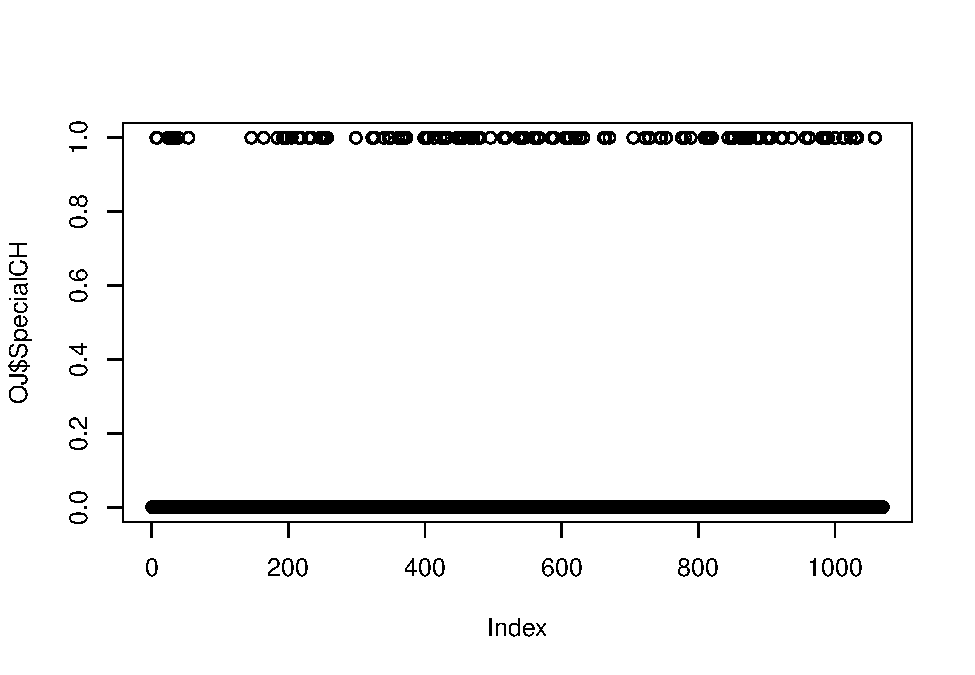
\includegraphics{durand_eltarr_files/figure-latex/unnamed-chunk-3-1.pdf}

\begin{Shaded}
\begin{Highlighting}[]
\KeywordTok{table}\NormalTok{(OJ}\OperatorTok{$}\NormalTok{SpecialMM)}
\end{Highlighting}
\end{Shaded}

\begin{verbatim}
## 
##   0   1 
## 897 173
\end{verbatim}

\begin{Shaded}
\begin{Highlighting}[]
\KeywordTok{plot}\NormalTok{(OJ}\OperatorTok{$}\NormalTok{SpecialMM)}
\end{Highlighting}
\end{Shaded}

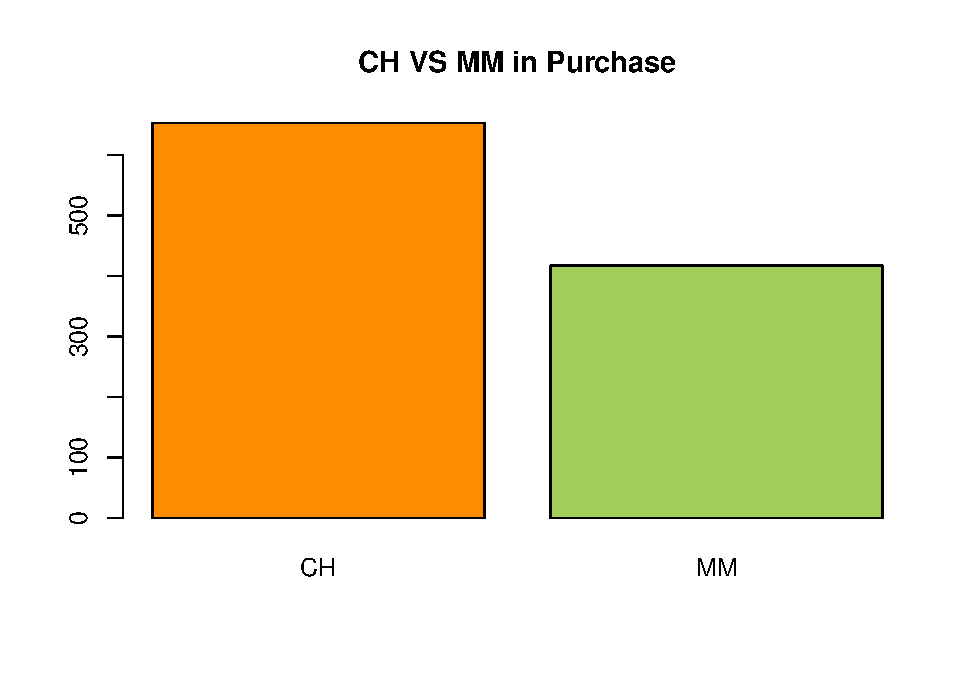
\includegraphics{durand_eltarr_files/figure-latex/unnamed-chunk-4-1.pdf}
De la même manière \(\texttt{STORE}\) ne prend que les valeurs entre 0
et 4.

\begin{Shaded}
\begin{Highlighting}[]
\KeywordTok{table}\NormalTok{(OJ}\OperatorTok{$}\NormalTok{STORE)}
\end{Highlighting}
\end{Shaded}

\begin{verbatim}
## 
##   0   1   2   3   4 
## 356 157 222 196 139
\end{verbatim}

\begin{Shaded}
\begin{Highlighting}[]
\KeywordTok{plot}\NormalTok{(OJ}\OperatorTok{$}\NormalTok{STORE)}
\end{Highlighting}
\end{Shaded}

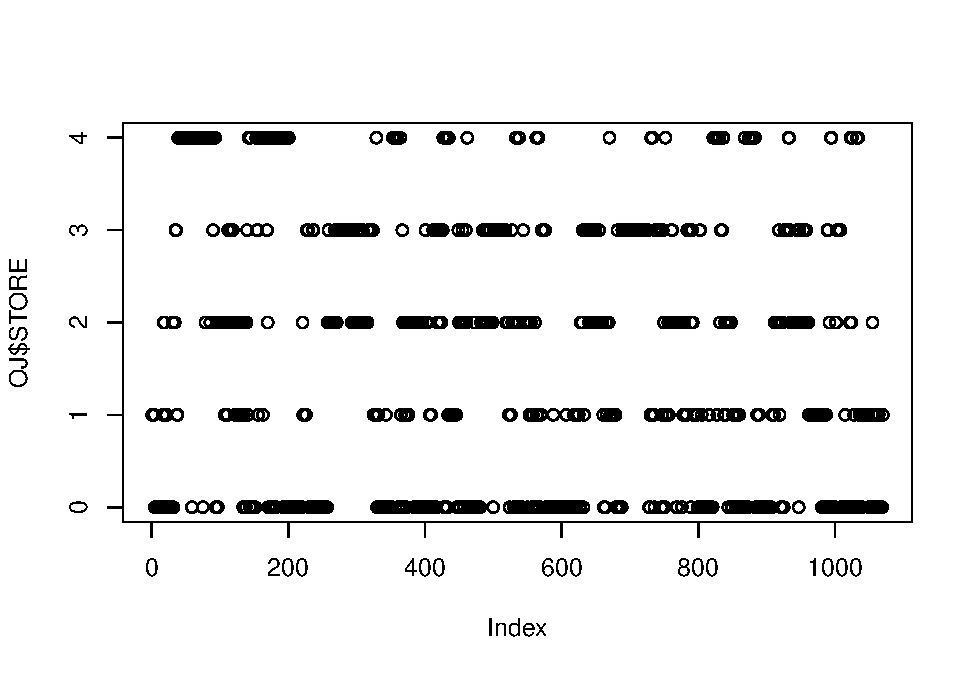
\includegraphics{durand_eltarr_files/figure-latex/unnamed-chunk-5-1.pdf}

On préfère alors les transformer en variables catégorielles:

\begin{Shaded}
\begin{Highlighting}[]
\NormalTok{OJ}\OperatorTok{$}\NormalTok{SpecialMM <-}\StringTok{ }\KeywordTok{as.factor}\NormalTok{(OJ}\OperatorTok{$}\NormalTok{SpecialMM)}
\NormalTok{OJ}\OperatorTok{$}\NormalTok{SpecialCH <-}\StringTok{ }\KeywordTok{as.factor}\NormalTok{(OJ}\OperatorTok{$}\NormalTok{SpecialCH)}
\NormalTok{OJ}\OperatorTok{$}\NormalTok{STORE <-}\StringTok{ }\KeywordTok{as.factor}\NormalTok{(OJ}\OperatorTok{$}\NormalTok{STORE}\OperatorTok{+}\DecValTok{1}\NormalTok{) }\CommentTok{## On préfère avoir des valeurs entre 1 et 5.}
\end{Highlighting}
\end{Shaded}

Ensuite, on voit que la variable \(\texttt{PriceDiff}\) est une
combinaison des deux variables \(\texttt{SalePriceMM}\) et
\(\texttt{SalePriceCH}\). On décide alors de la retrouver.

\begin{Shaded}
\begin{Highlighting}[]
\NormalTok{OJ <-}\StringTok{ }\KeywordTok{subset}\NormalTok{(OJ, }\DataTypeTok{select=}\OperatorTok{-}\NormalTok{PriceDiff)}
\end{Highlighting}
\end{Shaded}

\hypertarget{foruxeat-aluxe9atoires}{%
\section{Forêt aléatoires}\label{foruxeat-aluxe9atoires}}

Il faut tout d'abord changer la variable Class en variable factor :

\begin{Shaded}
\begin{Highlighting}[]
\NormalTok{email}\OperatorTok{$}\NormalTok{Class =}\StringTok{ }\KeywordTok{as.factor}\NormalTok{(email}\OperatorTok{$}\NormalTok{Class)}
\end{Highlighting}
\end{Shaded}

\hypertarget{question-4}{%
\subsection{Question 4}\label{question-4}}

\begin{Shaded}
\begin{Highlighting}[]
\KeywordTok{require}\NormalTok{(rpart)}
\end{Highlighting}
\end{Shaded}

\begin{verbatim}
## Loading required package: rpart
\end{verbatim}

\begin{Shaded}
\begin{Highlighting}[]
\KeywordTok{require}\NormalTok{(rpart.plot)}
\end{Highlighting}
\end{Shaded}

\begin{verbatim}
## Loading required package: rpart.plot
\end{verbatim}

\begin{verbatim}
## Warning: package 'rpart.plot' was built under R version 3.6.3
\end{verbatim}

\begin{Shaded}
\begin{Highlighting}[]
\KeywordTok{require}\NormalTok{(ipred)}
\end{Highlighting}
\end{Shaded}

\begin{verbatim}
## Loading required package: ipred
\end{verbatim}

\begin{verbatim}
## Warning: package 'ipred' was built under R version 3.6.3
\end{verbatim}

\begin{Shaded}
\begin{Highlighting}[]
\KeywordTok{require}\NormalTok{(caret)}
\end{Highlighting}
\end{Shaded}

\begin{verbatim}
## Loading required package: caret
\end{verbatim}

\begin{verbatim}
## Warning: package 'caret' was built under R version 3.6.3
\end{verbatim}

\begin{verbatim}
## Loading required package: lattice
\end{verbatim}

\begin{verbatim}
## Loading required package: ggplot2
\end{verbatim}

\begin{Shaded}
\begin{Highlighting}[]
\KeywordTok{require}\NormalTok{(randomForest)}
\end{Highlighting}
\end{Shaded}

\begin{verbatim}
## Loading required package: randomForest
\end{verbatim}

\begin{verbatim}
## Warning: package 'randomForest' was built under R version 3.6.3
\end{verbatim}

\begin{verbatim}
## randomForest 4.6-14
\end{verbatim}

\begin{verbatim}
## Type rfNews() to see new features/changes/bug fixes.
\end{verbatim}

\begin{verbatim}
## 
## Attaching package: 'randomForest'
\end{verbatim}

\begin{verbatim}
## The following object is masked from 'package:ggplot2':
## 
##     margin
\end{verbatim}

\begin{Shaded}
\begin{Highlighting}[]
\KeywordTok{require}\NormalTok{(doParallel)}
\end{Highlighting}
\end{Shaded}

\begin{verbatim}
## Loading required package: doParallel
\end{verbatim}

\begin{verbatim}
## Warning: package 'doParallel' was built under R version 3.6.3
\end{verbatim}

\begin{verbatim}
## Loading required package: foreach
\end{verbatim}

\begin{verbatim}
## Loading required package: iterators
\end{verbatim}

\begin{verbatim}
## Loading required package: parallel
\end{verbatim}

\begin{Shaded}
\begin{Highlighting}[]
\NormalTok{N =}\StringTok{ }\KeywordTok{nrow}\NormalTok{(email)}
\KeywordTok{set.seed}\NormalTok{(}\DecValTok{103}\NormalTok{)}
\NormalTok{train =}\StringTok{ }\KeywordTok{sample}\NormalTok{(}\DecValTok{1}\OperatorTok{:}\NormalTok{N, }\KeywordTok{round}\NormalTok{(}\FloatTok{0.75}\OperatorTok{*}\NormalTok{N))}
\NormalTok{email.tr =}\StringTok{ }\NormalTok{email[train,]}
\NormalTok{email.te =}\StringTok{ }\NormalTok{email[}\OperatorTok{-}\NormalTok{train,]}
\end{Highlighting}
\end{Shaded}

Ajustons tout d'abord un arbre sans élagage :

\begin{Shaded}
\begin{Highlighting}[]
\NormalTok{cart}\FloatTok{.0}\NormalTok{ <-}\StringTok{ }\KeywordTok{rpart}\NormalTok{(Class}\OperatorTok{~}\NormalTok{.,}
                \DataTypeTok{data=}\NormalTok{email.tr, }
                \DataTypeTok{control=}\KeywordTok{rpart.control}\NormalTok{(}\DataTypeTok{minsplit=}\DecValTok{1}\NormalTok{,}\DataTypeTok{cp=}\DecValTok{0}\NormalTok{, }\DataTypeTok{xval=}\DecValTok{30}\NormalTok{)) }\CommentTok{# minsplit=1,cp=0}
                                                                \CommentTok{# pour avoir un arbre le}
                                                                \CommentTok{# plus profond possible}
\KeywordTok{rpart.plot}\NormalTok{(cart}\FloatTok{.0}\NormalTok{)}
\end{Highlighting}
\end{Shaded}

\begin{verbatim}
## Warning: labs do not fit even at cex 0.15, there may be some overplotting
\end{verbatim}

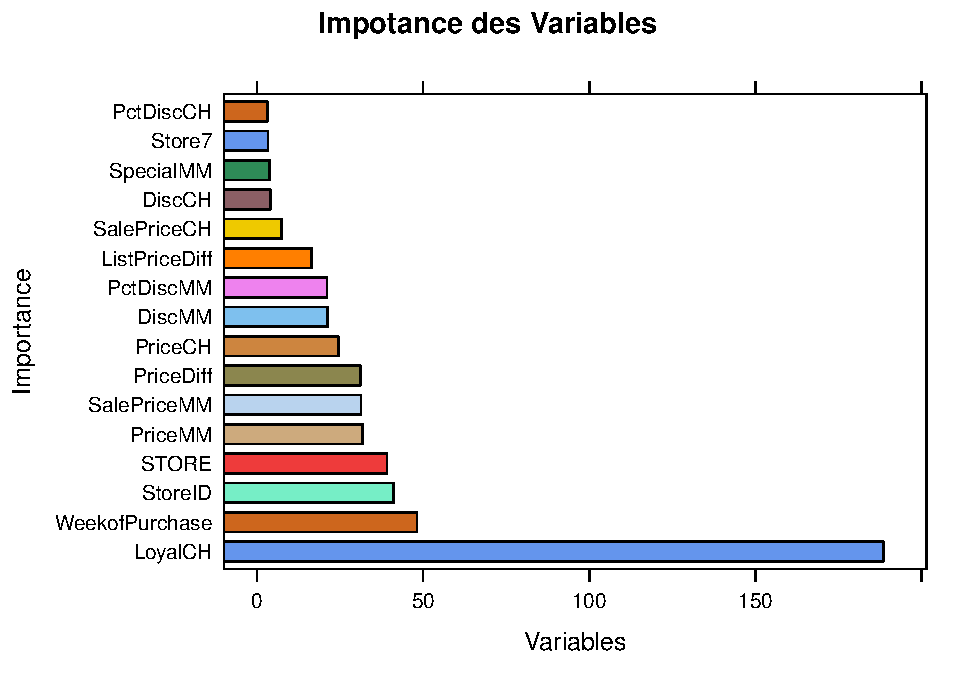
\includegraphics{durand_eltarr_files/figure-latex/unnamed-chunk-13-1.pdf}

Puis élagons cette arbre :

\begin{Shaded}
\begin{Highlighting}[]
\NormalTok{cart.pruned <-}\StringTok{ }\KeywordTok{prune}\NormalTok{(cart}\FloatTok{.0}\NormalTok{, }\DataTypeTok{cp =}\NormalTok{ cart}\FloatTok{.0}\OperatorTok{$}\NormalTok{cptable[}\KeywordTok{which.min}\NormalTok{(cart}\FloatTok{.0}\OperatorTok{$}\NormalTok{cptable[,}\StringTok{"xerror"}\NormalTok{]),}\StringTok{"CP"}\NormalTok{])}
\KeywordTok{rpart.plot}\NormalTok{(cart.pruned)}
\end{Highlighting}
\end{Shaded}

\begin{verbatim}
## Warning: labs do not fit even at cex 0.15, there may be some overplotting
\end{verbatim}

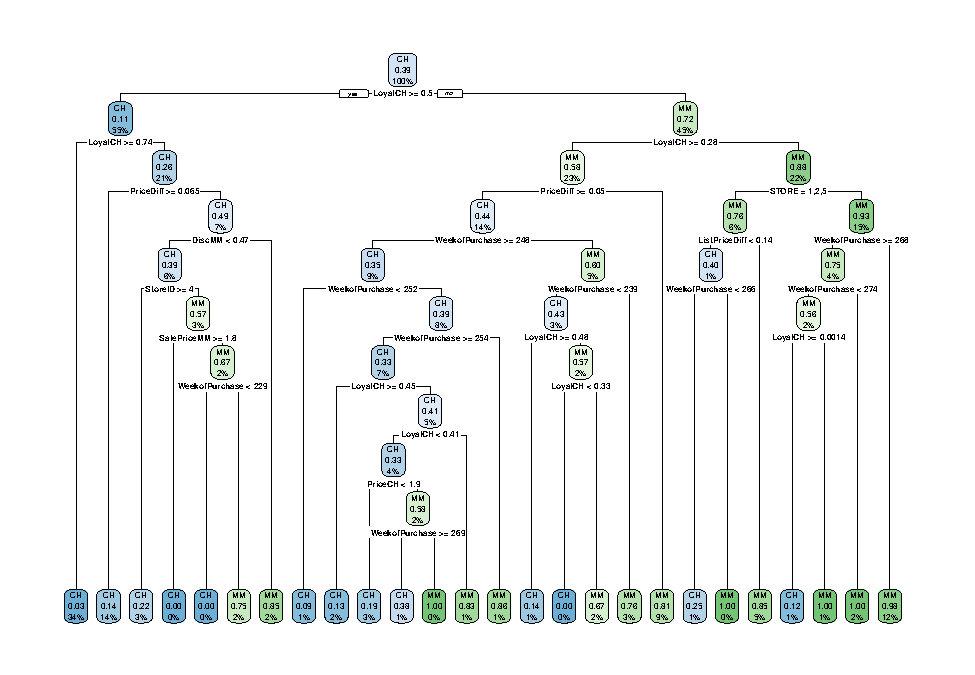
\includegraphics{durand_eltarr_files/figure-latex/unnamed-chunk-14-1.pdf}

Enfin on calcul l'erreur de test (taux de mauvais classement), en
appliquant la règle de Bayes :

\begin{Shaded}
\begin{Highlighting}[]
\NormalTok{pred.pruned <-}\StringTok{ }\KeywordTok{predict}\NormalTok{(cart.pruned, email.te)}
\KeywordTok{mean}\NormalTok{(}\KeywordTok{abs}\NormalTok{(}\KeywordTok{ifelse}\NormalTok{(email.te}\OperatorTok{$}\NormalTok{Class }\OperatorTok{==}\StringTok{ "Spam"}\NormalTok{, }\DecValTok{1}\NormalTok{,}\DecValTok{0}\NormalTok{) }\OperatorTok{-}\StringTok{ }\KeywordTok{ifelse}\NormalTok{(pred.pruned[,}\DecValTok{2}\NormalTok{] }\OperatorTok{>}\NormalTok{.}\DecValTok{5}\NormalTok{, }\DecValTok{1}\NormalTok{,}\DecValTok{0}\NormalTok{)))}
\end{Highlighting}
\end{Shaded}

\begin{verbatim}
## [1] 0.0773913
\end{verbatim}

Nous atteignons donc un taux de mauvais classement de 8\% avec ce
modèle.

Pour

\hypertarget{question-5}{%
\subsection{Question 5}\label{question-5}}

Nous réalisons un bagging 100 arbres de décisions à l'aide de la
fonction bagging de la librairie ipred :

\begin{Shaded}
\begin{Highlighting}[]
\NormalTok{bag.email <-}\StringTok{ }\KeywordTok{bagging}\NormalTok{(Class}\OperatorTok{~}\NormalTok{., }\DataTypeTok{data=}\NormalTok{email.tr, }\DataTypeTok{mfinal=}\DecValTok{100}\NormalTok{)}
\end{Highlighting}
\end{Shaded}

Puis on peut évaluer l'erreur de test :

\begin{Shaded}
\begin{Highlighting}[]
\NormalTok{pred.bag <-}\StringTok{ }\KeywordTok{predict}\NormalTok{(bag.email, email.te)}
\KeywordTok{mean}\NormalTok{(}\KeywordTok{abs}\NormalTok{(}\KeywordTok{ifelse}\NormalTok{(email.te}\OperatorTok{$}\NormalTok{Class }\OperatorTok{==}\StringTok{ "Spam"}\NormalTok{, }\DecValTok{1}\NormalTok{,}\DecValTok{0}\NormalTok{) }\OperatorTok{-}\StringTok{ }\KeywordTok{ifelse}\NormalTok{(pred.bag }\OperatorTok{==}\StringTok{ "Spam"}\NormalTok{, }\DecValTok{1}\NormalTok{,}\DecValTok{0}\NormalTok{)))}
\end{Highlighting}
\end{Shaded}

\begin{verbatim}
## [1] 0.04695652
\end{verbatim}

Nous avons donc une erreur de test de 7,5\%.

\hypertarget{question-6}{%
\subsection{Question 6}\label{question-6}}

Enfin, nous ajustons un modèle random forrest à 100 arbres en choisisant
le mtry, (c'est à dire le nombre de variable que l'on prend pour chaque
arbre), par validation croisée.

Le choix de mtry est reproductible grâce à la validation croisée.

Puis on peut évaluer l'erreur de test :

On a une erreur de test de 7\%.

\hypertarget{question-7}{%
\subsection{Question 7}\label{question-7}}

\hypertarget{autour-de-lalgorithme-adaboost}{%
\section{Autour de l'algorithme
Adaboost}\label{autour-de-lalgorithme-adaboost}}

\hypertarget{question-10}{%
\subsection{Question 10}\label{question-10}}

\[
\begin{tabular}{|l|M{4cm}|M{4cm}|M{4cm}|r|}
    \hline
     & &     Perte \\
     & & exponentielle & Perte binaire \\
     \hat{c}(x_*) & \hat{y}_* & exp(-y_* \hat{c}(x_*)) & 1(y_* \neq \hat{y}_*) & y_* \tabularnewline
    \hline
    0.3 & & & & -1
\tabularnewline
    \hline
    -0.2 & & & & -1
\tabularnewline
    \hline
    1.5 & & & & 1
\tabularnewline
    \hline
    -4.3 & & & & 1
\tabularnewline
    \hline
 \end{tabular}
\]

\end{document}
